\documentclass[a4paper, 10pt]{article}
\usepackage[margin=1in]{geometry} 
\usepackage{amsmath}
\usepackage{tcolorbox}
\usepackage{amssymb}
\usepackage{amsthm}
\usepackage{lastpage}
\usepackage{fancyhdr}
\usepackage{accents}
\usepackage{titlesec}

\usepackage{enumitem}
\setlist{nolistsep}

\usepackage[scaled]{helvet}
\renewcommand\familydefault{\sfdefault} 
\usepackage[T1]{fontenc}

\setlength{\parindent}{0pt}
\setlength{\parskip}{6pt}%

%parskip shold take care of heading spacing
\titlespacing\section{0pt}{0pt}{0pt}
\titlespacing\subsection{0pt}{0pt}{0pt}
\titlespacing\subsubsection{0pt}{0pt}{0pt}


\pagestyle{fancy}
\setlength{\headheight}{40pt}


\begin{document}

\lhead{ROHAN ANAND (19300059)} 
\rhead{CS7DS4 Data Visualization 2020 \\ Assignment 3} 
\cfoot{\thepage\ of \pageref{LastPage}}
\section{Introduction}

Visualizing data effectively can make it easier for users to analyse and understand data. Proper visualizations can also give better and new insights into data. Most visualizations are classified as either exploratory or explanatory in nature.

In this paper, we attempt to visualize the ``120 Years of Olympic History'' \cite{olympicDataset} Dataset over the years with the goal of exploring the relations of medals won. We also utilize the Worlds GDP dataset \cite{gdpDataset} to compare GDP with medals won. 

\section{Data Collection and Preprocessing}

The 2 datasets used were the ``120 Years of Olympic History'' and the Worlds GDP Dataset. The Olympics dataset contains information of athletes who participated in the Olympics from 1896 to 2016. It contains details of the athletes country and which medal they won. The GDP dataset contains the GDP in US dollars for each country from the year 1960 to 2016.

Before we can use these datasets together, they need to be combined. These datasets together have the ``Country'' as the common denominator, and were joined accordingly. Other preprocessing steps taken were standardizing country to ISO-3 standard and removing null values. All preprocessing was done using Python and Pandas.

\section{Visualization}

There are 3 core visualizations made in this paper:

\begin{enumerate}
	\item World Map of Olympic Medals over the years
	\item Pie Charts for distribution of medals for a particular country over the years
	\item Line Chart comparing GDP and Medals Won for a country
\end{enumerate}

All charts were created using Plotly \cite{plotly}. As such features of Plotly such as zooming, panning, scaling are made available for the user to interact with.

\subsection{World Map of Medals}

This is a visualization of the world and the medals won by each country. Each country has a bubble marker whose size represents the number of medals won. This plot is animated by the year and hence the size of these markers vary. The markers are color coded using the continent of the countries. On hovering over these markers, we see the information for medals won for that year. On clicking on one of the markers, the rest of the charts are generated according to which country that marker represents.

\begin{figure}[b]
\centering
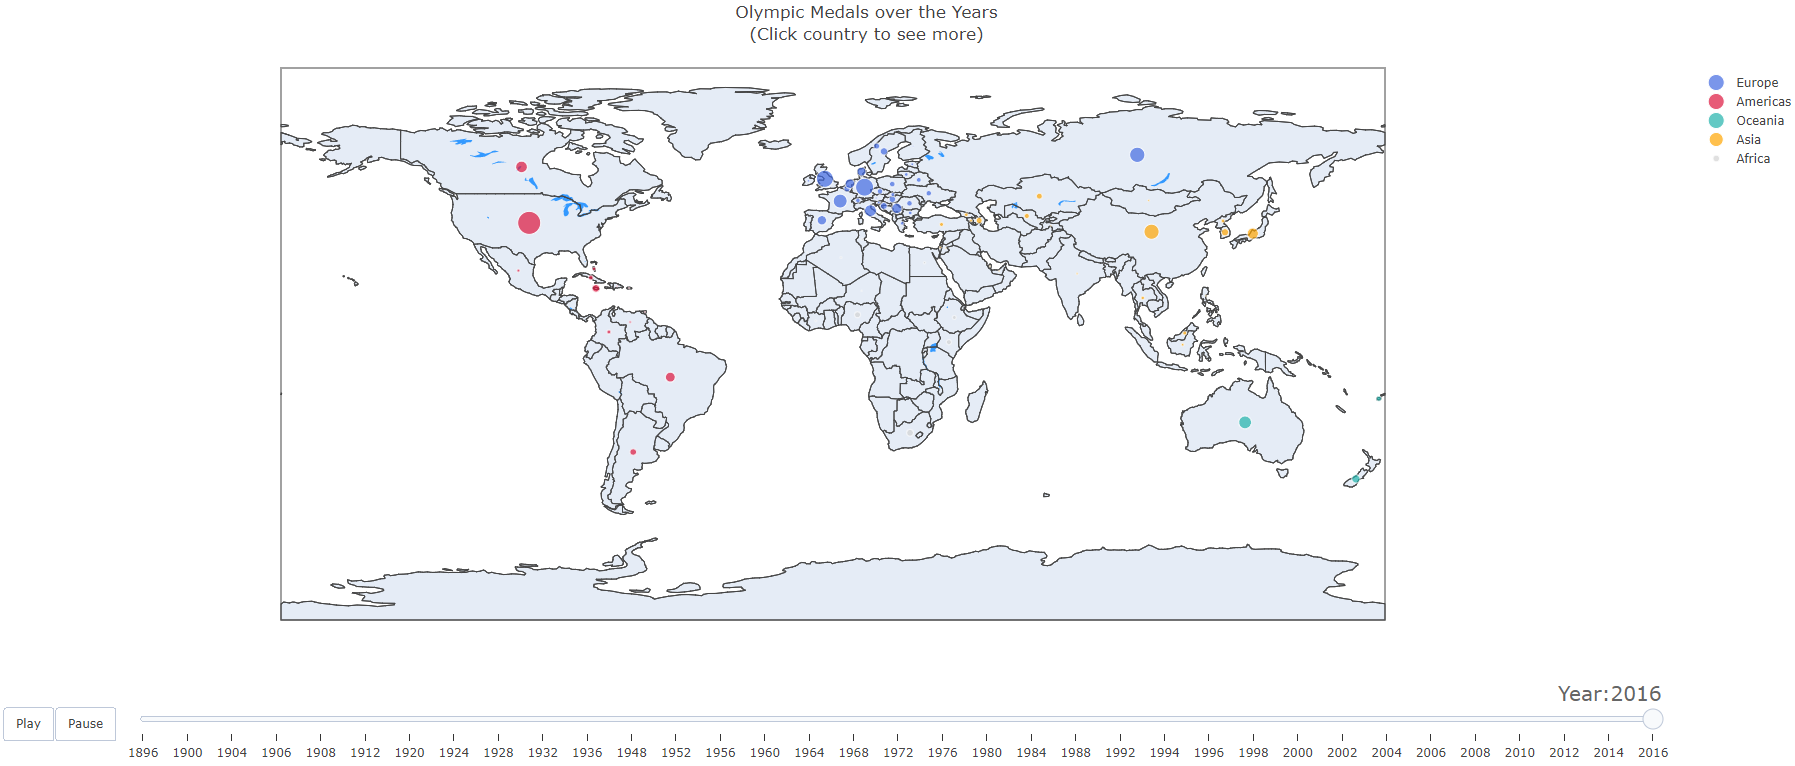
\includegraphics[scale=0.30]{map.png}
\caption{Map of Medals won over Time}
\end{figure}

\subsubsection{Datatypes}
The medal count and years are quantitative discrete values. Countries themselves are categorical/nominal values. The dataset is tabular.

\subsubsection{Tasks}
The goal of this visualization is to provide a broad understanding of the distribution of medals over the years. It also provides the interface for rendering other charts.

\subsubsection{Visual Encoding Channels}

\begin{itemize}
	\item Position: The position of the marker is based on the real country location.
	\item Size: The size of the marker changes based on the number of medals.
	\item Colour: The markers are colour coded by continents.
	\item Motion: The size of the marker is animated. 
\end{itemize}

\subsection{Pie Charts of Medal Distribution}

This chart contains multiple Pie charts in a sub-plot. Each sub-plot represents the distribution of medals won in a particular year for a country.

\begin{figure}[t]
\centering
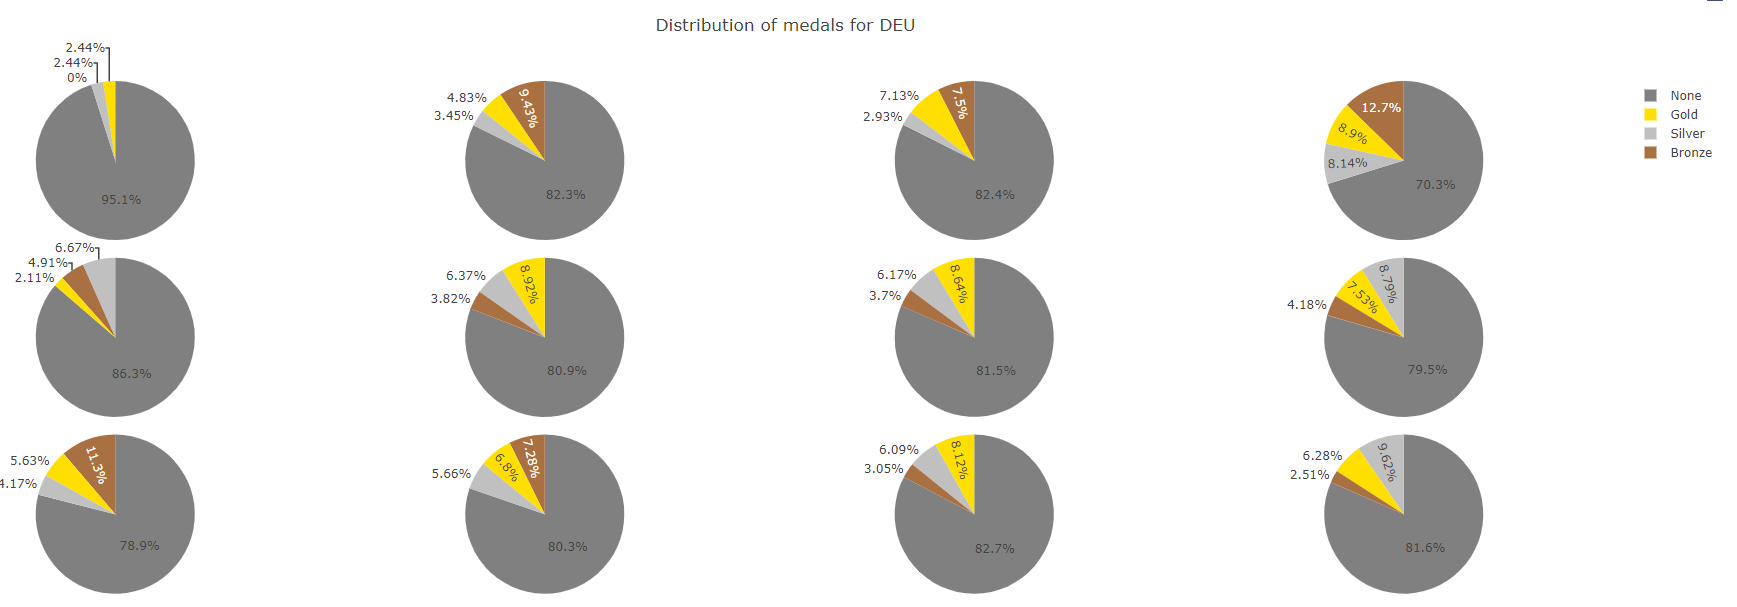
\includegraphics[scale=0.3]{pie.png}
\caption{Pie Charts of Distribution of medals}
\end{figure}

\subsubsection{Datatypes}
Each type of medal count is quantitative. The type of medals themselves are nominal. The dataset is tabular.

\subsubsection{Tasks}
This visualization provides an interface for the user to do an in depth analysis of the distribution of medals over the years.

\subsubsection{Visual Encoding Channels}

\begin{itemize}
	\item Position: The position of each chart is done by the year.
	\item Size: The area of each slice is determined by the number of medals.
	\item Colour: The slices are color coded based on the type of medal.
\end{itemize}

\subsection{Line Chart of GDP v.s. Medals}

This is a line chart of GDP and number of medals won for a country. It utilizes two Y-axis scales for GDP and Medals Won separately.

\begin{figure}[t]
\centering
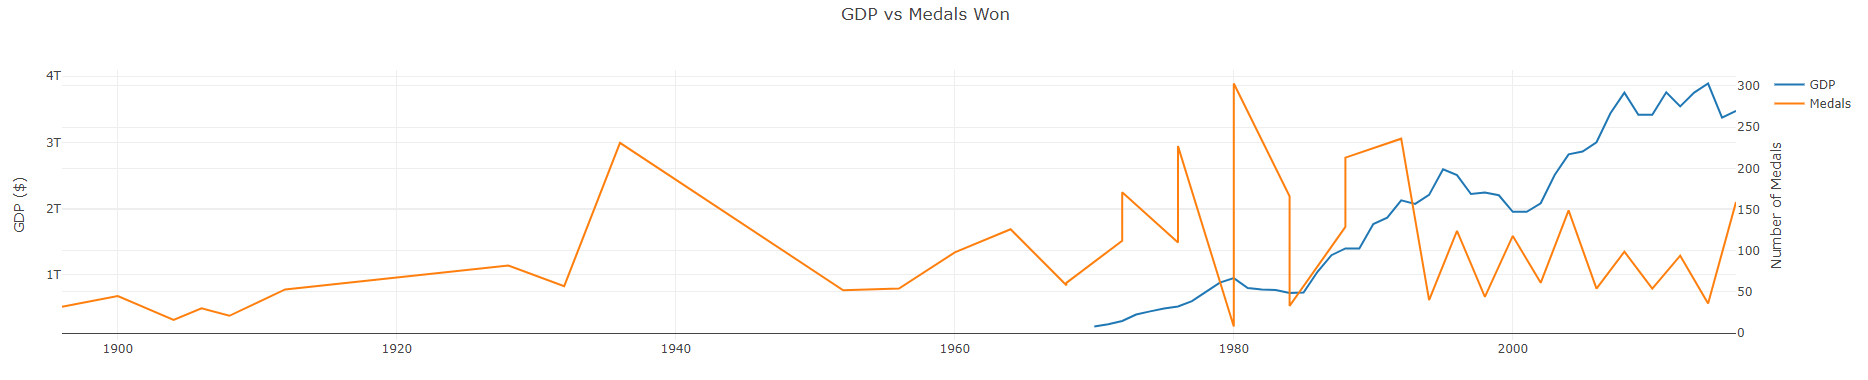
\includegraphics[scale=0.3]{line.png}
\caption{Line Chart of GDP versus Medals Count}
\end{figure}


\subsubsection{Datatypes}
Number of medals won and GDP is quantitative. The dataset is tabular.

\subsubsection{Tasks}
Using this chart, the user can attempt to discern if there is some pattern between GDP and medals won. 

\subsubsection{Visual Encoding Channels}

\begin{itemize}
	\item Colour: The line color is based on whether it represents GDP or Medals won.
\end{itemize}


% feel free to use bibtex
\begin{thebibliography}{9}

\bibitem{olympicDataset}
Griffin, R. ``120 Years of Olympic History: Athletes and Results.'' Accessed April 19, 2020. https://www.kaggle.com/heesoo37/120-years-of-olympic-history-athletes-and-results.

\bibitem{gdpDataset}
``Country, Regional and World GDP (Gross Domestic Product).'' Accessed April 19, 2020. https://datahub.io/core/gdp.

\bibitem{plotly}
``Plotly JS.'' Accessed April 19, 2020. https://plotly.com/javascript/.
\end{thebibliography}
\label{LastPage}

\end{document}
